\documentclass[12pt, titlepage]{article}

\usepackage{booktabs}
\usepackage{tabularx}
\usepackage{hyperref}
\usepackage{pdflscape}
\usepackage{graphicx}
\hypersetup{
    colorlinks,
    citecolor=blue,
    filecolor=black,
    linkcolor=red,
    urlcolor=blue
}
\usepackage[round]{natbib}

%% Comments

\usepackage{color}

\newif\ifcomments\commentstrue %displays comments
%\newif\ifcomments\commentsfalse %so that comments do not display

\ifcomments
\newcommand{\authornote}[3]{\textcolor{#1}{[#3 ---#2]}}
\newcommand{\todo}[1]{\textcolor{red}{[TODO: #1]}}
\else
\newcommand{\authornote}[3]{}
\newcommand{\todo}[1]{}
\fi

\newcommand{\wss}[1]{\authornote{blue}{SS}{#1}} 
\newcommand{\plt}[1]{\authornote{magenta}{TPLT}{#1}} %For explanation of the template
\newcommand{\an}[1]{\authornote{cyan}{Author}{#1}}

%% Common Parts

\newcommand{\progname}{ProgName} % PUT YOUR PROGRAM NAME HERE
\newcommand{\authname}{Team \#, Team Name
\\ Student 1 name
\\ Student 2 name
\\ Student 3 name
\\ Student 4 name} % AUTHOR NAMES                  

\usepackage{hyperref}
    \hypersetup{colorlinks=true, linkcolor=blue, citecolor=blue, filecolor=blue,
                urlcolor=blue, unicode=false}
    \urlstyle{same}
                                


\begin{document}

\title{System Verification and Validation Plan for \progname{}} 
\author{\authname}
\date{\today}
	
\maketitle

\pagenumbering{roman}

\section*{Revision History}

\begin{tabularx}{\textwidth}{p{3cm}p{2cm}X}
\toprule {\bf Date} & {\bf Version} & {\bf Notes}\\
\midrule
2025-02-24 & 1.0 & Initial Release\\
\bottomrule
\end{tabularx}

~\\
\wss{The intention of the VnV plan is to increase confidence in the software.
However, this does not mean listing every verification and validation technique
that has ever been devised.  The VnV plan should also be a \textbf{feasible}
plan. Execution of the plan should be possible with the time and team available.
If the full plan cannot be completed during the time available, it can either be
modified to ``fake it'', or a better solution is to add a section describing
what work has been completed and what work is still planned for the future.}

\wss{The VnV plan is typically started after the requirements stage, but before
the design stage.  This means that the sections related to unit testing cannot
initially be completed.  The sections will be filled in after the design stage
is complete.  the final version of the VnV plan should have all sections filled
in.}

\newpage

\tableofcontents

\listoftables
\wss{Remove this section if it isn't needed}

\listoffigures
\wss{Remove this section if it isn't needed}

\newpage

\section{Symbols, Abbreviations, and Acronyms}

\renewcommand{\arraystretch}{1.2}
\begin{tabular}{l l} 
  \toprule		
  \textbf{symbol} & \textbf{description}\\
  \midrule
  FOV & Field-of-view\\
  $\mathcal{I}(x,y)$ & 2D array of pixel values for a greyscale image \\
  $i$ & total number of robot poses\\
  $j$ & total number of cameras\\
  $K$ & array of identified keypoints\\
  $k$ & number of total keypoints\\
  $m$ & horizontal image size\\
  $n$ & vertical image size\\
  ORB & Oriented FAST and Rotated BRIEF\\
  SRS & Software Requirements Specification\\
  VnV & Verification and Validation\\
  $\sigma$ & standard deviation\\
  \bottomrule
\end{tabular}\\

\newpage

\pagenumbering{arabic}

The intent of this document is to define the verification and validation process 
that will be used to assess the feature correspondence software from camera 
imagery. Specifically, this document will be used to characterize the behaviour and 
performance of this software. The remaining section of this document outline a high 
level summary of the general system system and specific objects of the VnV process. 
It also defines specific strategies for the individual verification plans, an overview of 
anticipated system tests, and an outline of specific unit test cases.

\section{General Information}

\subsection{Summary}
Image Feature Correspondences (IFC) is a feature comparison algorithm that is intended 
to be used as part of a pipeline to perform extrinsic camera calibration for 
applications in mobile robotics. It accepts camera intrinsics and imagery data at different 
poses to identify common features across collected images. 

\subsection{Objectives}
The VnV process is intended to characterize how well the for the IFC software performs in its 
intended capacity to identify features amongst collected imagery. This can vary significantly 
as it is influenced by factors such as overlap in camera fields-of-view (FOV), contrast 
between objects in an image, and variance in either scale or rotation. Furthermore, as there is 
no common baseline to compare this software to as an oracle model,  the intent of the VnV for 
the IFC software is to characterize the performance of the integrated image processing functions 
against a set of selected datasets. Key objectives of this process are defined below.
\begin{itemize}
  \item correctness of feature extraction
  \item correctness of feature comparison
  \item assessment of scale variance between features
  \item assessment of rotation variance between features
  \item benchmarking of processing time and memory usage for large image strategies
  \item cross-validation of system performance with accepted benchmarked datasets
\end{itemize}

Characterization of the individual functions within the OpenCV library themselves remains outside of the scope of 
this project, as we can assume that the library has been verified by uts own 
implementation team. 
\\ \\

\subsection{Challenge Level and Extras}

\wss{State the challenge level (advanced, general, basic) for your project.
Your challenge level should exactly match what is included in your problem
statement.  This should be the challenge level agreed on between you and the
course instructor.  You can use a pull request to update your challenge level
(in TeamComposition.csv or Repos.csv) if your plan changes as a result of the
VnV planning exercise.}

\wss{Summarize the extras (if any) that were tackled by this project.  Extras
can include usability testing, code walkthroughs, \textcolor{red}{\textbf{user documentation}}, formal
proof, GenderMag personas, Design Thinking, etc.  Extras should have already
been approved by the course instructor as included in your problem statement.
You can use a pull request to update your extras (in TeamComposition.csv or
Repos.csv) if your plan changes as a result of the VnV planning exercise.}\\
\textcolor{red}{\textbf{Discuss with Project Instructor.}}

\subsection{Relevant Documentation}

Relevant documentation has been hyperlinked throughout the length of the document. This enables 
the reader to access each resource within the context of the section that the reference is 
invoked.

\section{Plan}
This section outlines how each aspect of the VnV effort will be performed. It outlines the 
different roles of reviewers adn the methods for which feedback will be collected and 
addressed.

\subsection{Verification and Validation Team}
The VnV team consists of four members, each of whom play a distinct role in the 
verification process.\\
\begin{tabular}{|p{0.11\linewidth}|p{0.24\linewidth}|p{0.6\linewidth}|} 
  \hline
  \textbf{Name} & \textbf{Role} & \textbf{Description}\\
  \hline
  Kiran Singh & Lead Developer and Test Designer & Responsibilities include 
  identification of key business cases for integrated tests,  design and 
  implementation of module tests, unit tests, and documentation of test 
  results\\
  \hline
  Matthew Giamou & Project Supervisor & Lead consultant on integrated 
  performance needs and decomposition for software modules. Responsibilities 
  include review of proposed VnV scope, approval of test cases as proposed by 
  Kiran S., and provision of feedback as to whether the test cases need to be 
  redefined within the scope of the full implementation of the IFC\\
  \hline
  Aliyah Jimoh & Domain Expert & Responsibilities include provision of 
  feedback on proposed test cases for the 
  scope of test cases for both the functional and non-functional requirements 
  as an reviewer that is less familiar with the overall implementation of the 
  system that its primary developer\\
  \hline
  Spencer Smith & Software Development Instructor & Responsibilities include 
  provision of feedback on proposed test cases for the scope of test cases 
  for both the functional and non-functional requirements as an reviewer that 
  is less familiar with the application domain of the system than all other 
  reviewers\\
  \bottomrule
\end{tabular}\\

\subsection{SRS Verification Plan}
The \textbf{\href{https://github.com/KiranSingh15/CAS-741-Image-Correspondences/blob/main/docs/SRS/SRS.pdf}
{SRS}} shall be reviewed by each member of the reviewer team to form consensus that the SRS has been correctly 
decomposed into sufficient requirements.\\
\begin{itemize}
\item the models are deemed to be comprehensible
\item the models are deemed to be correct
\item the associated requirements are traced correctly with respect to the models 
and project scope 
\item the requirements are decomposed in a manner that facilitates verification
\end{itemize}
Feedback on the SRS from the Domain Expert and Instructor will be captured through 
the use of Github Issues. Specifically, both reviewers will use the 
\textbf{\href{https://github.com/KiranSingh15/CAS-741-Image-Correspondences/blob/
main/docs/Checklists/SRS-Checklist.pdf}
{SRS Checklist}}. 
The lead developer will respond in turn to each issue and if 
reserves the right to reject a proposed change as needed. \\ \\
The Lead Developer will schedule a meeting with the Project Supervisor to walk through 
the first revision of the SRS document. In this meeting, the Project Supervisor will offer 
feedback and recommendations for candidate revisions to the outlined models and requirements. 
The Lead Developer will then prepare issues in Github to address each proposed revision. \\ \\

\subsection{Design Verification Plan}
The Domain Expert and Course Instructor will review the Module Guide 
\textbf{\href{https://github.com/KiranSingh15/CAS-741-Image-Correspondences/blob/main/docs/Design/SoftArchitecture/MG.pdf}
{(MG)}} and the Module Interface Specification 
\textbf{\href{https://github.com/KiranSingh15/CAS-741-Image-Correspondences/blob/main/docs/Design/SoftDetailedDes/MIS.pdf}
{(MIS)}} against the 
\textbf{\href{https://github.com/KiranSingh15/CAS-741-Image-Correspondences/blob/main/docs/Checklists/MG-Checklist.pdf}
{MG}} and
\textbf{\href{https://github.com/KiranSingh15/CAS-741-Image-Correspondences/blob/main/docs/Checklists/MIS-Checklist.pdf}
{MIS}} checklists. The intent of this process is to ensure that the design of of the system is:
\begin{enumerate}
\item unambiguous
\item adheres to best-practices of module design
\item aligns with the requirements as identified in the 
\textbf{\href{https://github.com/KiranSingh15/CAS-741-Image-Correspondences/blob/main/docs/SRS/SRS.pdf}
{SRS}}
\end{enumerate}


\subsection{Verification and Validation Plan Verification Plan}
The VnV Plan will be verified via inspection by the Domain Expert and the 
Software Development Instructor. The 
\textbf{\href{https://github.com/KiranSingh15/CAS-741-Image-Correspondences/blob/main/docs/Checklists/SRS-Checklist.pdf}
{VnV Plan Checklist}} 
will be used as the assessment criteria for the inspection. 
Feedback will provided as Github issues and will be handled in the same manner as feedback 
for the SRS.\\ \\
Mutation testing will be performed against the test outlined in Section \ref{UTD}.

\subsection{Implementation Verification Plan}
The IFC software shall be verified against the test procedures outlined in Sections \ref{FR_Tests} and 
\ref{NFR_Tests}. Static verification of the IFC software will consist of a code walkthrough. This will take 
place during the CAS 741 final presentation, where the Domain Expert and Course Instructor in the 
will have the opportunity to observed the code and raise issues following the presentation via GitHub. \\ \\
Dynamic  verification of the IFC software will consist of system and unit tests via PyTest. System tests 
are outlined in Section \ref{Sys_Tests}. Unit tests will be outlined in Rev 2 of the VnV Plan in 
Section \ref{UTD}.

\subsection{Automated Testing and Verification Tools}
Several tools will be used to support automated testing and verification. They include:
\begin{itemize}
\item Continuous Integration (CI) will be facilitated via GitHub Actions. A pull request will be used 
to run automated tests.
\item Pytest will be used to perform system tests, unit tests, and to assess code coverage. 
\item flake8 will be used as a linter to ensure adherence to PEP8 standards. 
\item PyLint, as an alternative linter to flake8.
\end{itemize}

\subsection{Software Validation Plan}
\wss{If there is any external data that can be used for validation, you should
  point to it here.  If there are no plans for validation, you should state that
  here.}
\wss{You might want to use review sessions with the stakeholder to check that
the requirements document captures the right requirements.  Maybe task based
inspection?}\\ \\

\textcolor{red}{The IFC software will be compared against benchmark data from \textbf{[INSERT DATASET HERE]} 
to characterize its performance.}


\section{System Tests}\label{Sys_Tests}
This section outlines the general roadmap for the required integrated system tests. 
\subsection{Tests for Functional Requirements} \label{FR_Tests}
This section outlines the system tests that verify the requirements outlined in 
Section 5 of the 
\textbf{\href{https://github.com/KiranSingh15/CAS-741-Image-Correspondences/blob/main/docs/SRS/SRS.pdf}
{SRS}}. 

\begin{figure}[h!]
  \begin{center}
   
\includegraphics[width=0.6\textwidth]{images/ArUco_Field_Gen.jpg}
  \caption{An example of a generated ArUco pattern. Image taken from \cite{ARUCO_Markers_openCV}}
  \label{gen_aruco} 
  \end{center}
\end{figure}

\begin{figure}[h!]
  \begin{center}
   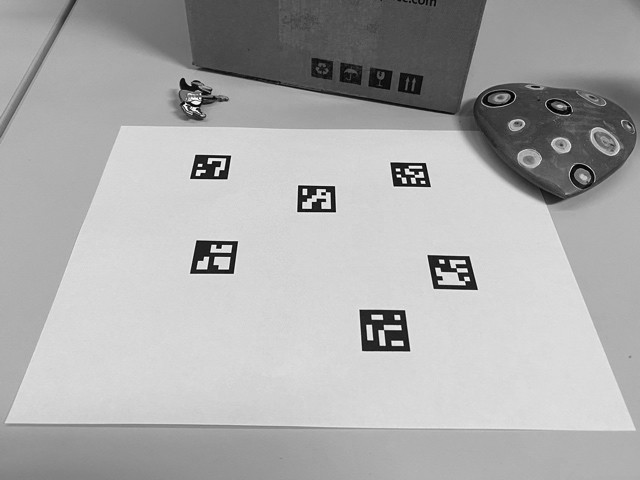
\includegraphics[width=0.6\textwidth]{images/GS_ArUco_Field_Image.jpg}
  \caption{An example of ArUco patterns within the scene of a captured greyscale image. 
  Image taken from \cite{ARUCO_Markers_openCV}}
  \label{gs_aruco_field} 
  \end{center}
\end{figure}

\subsubsection{Feature Detection}
This test section is intended to assess that the system can accept new parameters from users and covers 
requirements R1 through R7 and R9 through R11, in Section 5.1 of the 
\textbf{\href{https://github.com/KiranSingh15/CAS-741-Image-Correspondences/blob/main/docs/SRS/SRS.pdf}
{SRS}}. 
		
\paragraph{Image Smoother}
\begin{enumerate}
\item \hypertarget{FT-IS-01}{FT-IS-01}
Control: Automated		

Initial State: Uninitialized

Input: A collection of 20 images $I$, each defined as 2D array of specified resolution, that contain 
binary patterned fiducial markers, named 
\href{https://docs.opencv.org/4.x/d5/dae/tutorial_aruco_detection.html}
{ArUco} markers (Figure \ref{gen_aruco}), within the image scene as demonstrated 
in Figure \ref{gs_aruco_field}. The user will also assign the image intensity standard deviation $\sigma$ to define the 
size of the Gaussian Kernel.

Output: 20 output images as a 2D array, each of which have a descriptive name that clearly identifies the 
input image from which it originates. The $I'$ array should be of equal size and the same data type as its 
corresponding image $I$. All images should be saved under its own uniquely named folder to prevent mixing 
of input and output imagery.

How test will be performed: Automated Tools (i.e. Pytest)

\end{enumerate}


\paragraph{Keypoint Detector}
\begin{enumerate}
\item \hypertarget{FT-KP-01}{FT-KP-01\\}
Control: Automatic	

Initial State: Uninitialized			

Input: A collection of 20 smoothed images $I'$, each defined as 2D array of specified resolution, that contain 
binary patterned fiducial markers as outlined in System Test \hyperlink{FT-IS-01}{FT-IS-01}. 
Permissible image intensity threshold, $t$.

Output: $K$: A 2D array of size $n \times 2$, where $n$ is the quantity of identified keypoints, 
where the first and second columns are populated with the horizontal and vertical coordinates for each 
keypoint. Each entry in the array should be an integer value. Each array should have a unique identifier that 
clearly defines the original image from which its keypoints were identified. All output arrays should be saved 
to a unique folder to separate them from the input images.

How test will be performed: Automated Tools (i.e. Pytest)
\end{enumerate}

\paragraph{Feature Definition}
\begin{enumerate}
\item \hypertarget{FT-FD-01}{FT-FD-01\\}
Control: Automatic

Initial State: Uninitialized

Input: A collection of 20 images, each defined as a 2D array of integers, and a collection of 20 $n\times 2$ 2D arrays, where n is the number of 
keypoints and is specific to each image. A patch size, $s$, will also be input as a scalar integer to define the the region for which to search for 
descriptors. A target number of descriptors, titled $d_{total}$, will also be input as a non-negative integer between 1 and 1023.

Output: $D_{bin}$, a 1D array of length $d_total$ where all entries of the array are 32 byte binary strings. 

Test Case Derivation: Source: \href{https://sites.cc.gatech.edu/classes/AY2024/cs4475_summer/images/ORB_an_efficient_alternative_to_SIFT_or_SURF.pdf}
{ORB: An efficient alternative to SIFT or SURF}. The preceding publication outlines methods 
to develop and the corresponding assessment of binary feature descriptors.

How test will be performed: Automated Tools (i.e. Pytest)
\end{enumerate}

\subsubsection{Feature Comparison}

This test section is intended to assess that the system can accept new parameters from users and covers 
requirements \textcolor{red}{R8 and R12 through R15} in Section 5.1 of the 
\textbf{\href{https://github.com/KiranSingh15/CAS-741-Image-Correspondences/blob/main/docs/SRS/SRS.pdf}
{SRS}}. 
		
\paragraph{Descriptor Comparison}
\begin{enumerate}
\item \hypertarget{FT-DC-01}{FT-DC-01\\}
Control: Automated		

Initial State: Uninitialized

Input: A total of 20 1D arrays, each of which may have a unique length, where each element of the 
array is a 32 byte binary strings known as a binary descriptor. Each array should be labeled with a descriptive 
name that outlines the instance of both the camera and pose at the time of image capture.

Output: A dynamically-sized array where the length, of the array is the number of matched features. The columns 
of the array will include the parameters as follows.
\begin{itemize}
\item Binary descriptors of both features as 32 byte binary strings
\item Corresponding image IDs for each feature
\item Matching scores between both features
\end{itemize}

How test will be performed: Automated Tools (i.e. Pytest)
\end{enumerate}

\subsection{Tests for Nonfunctional Requirements}\label{NFR_Tests}
The only non-functional requirement outlined in the 
\textbf{\href{https://github.com/KiranSingh15/CAS-741-Image-Correspondences/blob/main/docs/SRS/SRS.pdf}
{SRS}} is NFR.1, which outlines that the system should be compatible with Python 3.1 libraries. 
This will be achieved by the walkthrough of each code module that will take place during the 
final CAS 703 presentation. An additional code walkthrough will be provided exclusively for
the Project Supervisor their request.

\newpage
\subsection{Traceability Between Test Cases and Requirements}
\begin{table}[h!]
  \centering
  \begin{tabular}{|c|c|c|c|c|}
  \hline
    Reqt\textbackslash Test & FT-IS-01 & FT-KP-01 & FT-FD-01 & FT-FC-01\\
  \hline
  R1    &X& & & \\ \hline
  R2    & &X& & \\ \hline
  R3    & & &X& \\ \hline
  R4    & & &X& \\ \hline
  R5    &X& & & \\ \hline
  R6    & &X& & \\ \hline
  R7    & & &X& \\ \hline
  R8    & & & &X\\ \hline
  R9    &X& & & \\ \hline
  R10   & &X& & \\ \hline
  R11   & & &X& \\ \hline
  R12   & & & &X\\ \hline
  R13   & & & &X\\ \hline
  R14   & & & &X\\ \hline
  R15   & & & &X\\ \hline
  NFR1  &O&O&O&O\\ \hline
  \hline
  \end{tabular}
  \caption{Traceability Matrix Showing the Connections Between Requirements and Instance Models}
  \label{Table:R_trace}
\end{table}

\begin{itemize}
\item X indicates a direct method of verification
\item O indicates an indirect method of verification, in tangent to a code walkthrough
\end{itemize}


\section{Unit Test Description}\label{UTD}

\wss{This section should not be filled in until after the MIS (detailed design
  document) has been completed.}

\wss{Reference your MIS (detailed design document) and explain your overall
philosophy for test case selection.}  

\wss{To save space and time, it may be an option to provide less detail in this section.  
For the unit tests you can potentially layout your testing strategy here.  That is, you 
can explain how tests will be selected for each module.  For instance, your test building 
approach could be test cases for each access program, including one test for normal behaviour 
and as many tests as needed for edge cases.  Rather than create the details of the input 
and output here, you could point to the unit testing code.  For this to work, you code 
needs to be well-documented, with meaningful names for all of the tests.}

\subsection{Unit Testing Scope}

\wss{What modules are outside of the scope.  If there are modules that are
  developed by someone else, then you would say here if you aren't planning on
  verifying them.  There may also be modules that are part of your software, but
  have a lower priority for verification than others.  If this is the case,
  explain your rationale for the ranking of module importance.}

\subsection{Tests for Functional Requirements}

\wss{Most of the verification will be through automated unit testing.  If
  appropriate specific modules can be verified by a non-testing based
  technique.  That can also be documented in this section.}

\subsubsection{Module 1}

\wss{Include a blurb here to explain why the subsections below cover the module.
  References to the MIS would be good.  You will want tests from a black box
  perspective and from a white box perspective.  Explain to the reader how the
  tests were selected.}

\begin{enumerate}

\item{test-id1\\}

Type: \wss{Functional, Dynamic, Manual, Automatic, Static etc. Most will
  be automatic}
					
Initial State: 
					
Input: 
					
Output: \wss{The expected result for the given inputs}

Test Case Derivation: \wss{Justify the expected value given in the Output field}

How test will be performed: 
					
\item{test-id2\\}

Type: \wss{Functional, Dynamic, Manual, Automatic, Static etc. Most will
  be automatic}
					
Initial State: 
					
Input: 
					
Output: \wss{The expected result for the given inputs}

Test Case Derivation: \wss{Justify the expected value given in the Output field}

How test will be performed: 

\item{...\\}
    
\end{enumerate}

\subsubsection{Module 2}

...

\subsection{Tests for Nonfunctional Requirements}

\wss{If there is a module that needs to be independently assessed for
  performance, those test cases can go here.  In some projects, planning for
  nonfunctional tests of units will not be that relevant.}

\wss{These tests may involve collecting performance data from previously
  mentioned functional tests.}

\subsubsection{Module ?}
		
\begin{enumerate}

\item{test-id1\\}

Type: \wss{Functional, Dynamic, Manual, Automatic, Static etc. Most will
  be automatic}
					
Initial State: 
					
Input/Condition: 
					
Output/Result: 
					
How test will be performed: 
					
\item{test-id2\\}

Type: Functional, Dynamic, Manual, Static etc.
					
Initial State: 
					
Input: 
					
Output: 
					
How test will be performed: 

\end{enumerate}

\subsubsection{Module ?}

...

\subsection{Traceability Between Test Cases and Modules}

\wss{Provide evidence that all of the modules have been considered.}
				
\bibliographystyle{plainnat}

\bibliography{../../refs/References}

\newpage

\section{Appendix}

This is where you can place additional information.

\subsection{Symbolic Parameters}

The definition of the test cases will call for SYMBOLIC\_CONSTANTS.
Their values are defined in this section for easy maintenance.

\newpage{}
\centering
End of document.
\end{document}